\providecommand{\setflag}{\newif \ifwhole \wholefalse}
\setflag
\ifwhole\else

% Typography and geometry ----------------------------------------------------
\documentclass[letterpaper]{scrbook}
\usepackage[inner=3cm,top=2.5cm,outer=3.5cm]{geometry}

\renewcommand\familydefault{bch}
\usepackage[utf8]{inputenc}
\usepackage{microtype}
\usepackage[small]{caption}
\usepackage[small]{titlesec}
\raggedbottom

% Graphics -------------------------------------------------------------------
\usepackage[pdftex]{graphicx}
\graphicspath{{_include/}}
\DeclareGraphicsExtensions{.png,.pdf}

% Code formatting ------------------------------------------------------------
\usepackage{fancyvrb}
\usepackage{courier}
\usepackage{listings}
\usepackage{color}
\usepackage{alltt}


\definecolor{comment}{rgb}{0.60, 0.60, 0.53}
\definecolor{background}{rgb}{0.97, 0.97, 1.00}
\definecolor{string}{rgb}{0.863, 0.066, 0.266}
\definecolor{number}{rgb}{0.0, 0.6, 0.6}
\definecolor{variable}{rgb}{0.00, 0.52, 0.70}
\lstset{
  basicstyle=\ttfamily,
  keywordstyle=\bfseries, 
  identifierstyle=,  
  commentstyle=\color{comment} \emph,
  stringstyle=\color{string},
  showstringspaces=false,
  columns = fullflexible,
  backgroundcolor=\color{background},
  mathescape = true,
  escapeinside=&&,
  fancyvrb
}
\newcommand{\code}[1]{\lstinline!#1!}
\newcommand{\f}[1]{\lstinline!#1()!}



% Links ----------------------------------------------------------------------

\usepackage{hyperref}
\definecolor{slateblue}{rgb}{0.07,0.07,0.488}
\hypersetup{colorlinks=true,linkcolor=slateblue,anchorcolor=slateblue,citecolor=slateblue,filecolor=slateblue,urlcolor=slateblue,bookmarksnumbered=true,pdfview=FitB}
\usepackage{url}

% Tables ---------------------------------------------------------------------
\usepackage{longtable}
\usepackage{booktabs}

% Miscellaneous --------------------------------------------------------------
\usepackage{pdfsync}
\usepackage{appendix}

\usepackage[round,sort&compress,sectionbib]{natbib}
\bibliographystyle{plainnat}


\title{ggplot2}
\author{Hadley Wickham}

\begin{document}
\fi


\chapter{Aesthetic specifications}
\label{cha:aesthetic_specifications}

\section{Introduction}

Summary in one place of the information available in \code{?par}.

\section{Colour}
\label{sec:colour_spec}

Colours can be specified in several different ways. 

\begin{itemize}
  \item In terms of {\bf rgb components}, with a string of the form \code{"#RRGGBB"} where each of the pairs \code{RR}, \code{GG}, \code{BB} consist of two hexadecimal digits giving a value in the range \code{00} to \code{FF}. 

  \item A {\bf name}, e.g.\ \code{"red"}. The colours are displayed in Figure~\ref{fig:colours}, and can be listed in more detail with \f{colours}. The Stower's institute provides a nice printable pdf that lists all colours:  \url{http://research.stowers-institute.org/efg/R/Color/Chart/}.
    
  \item An {\bf NA}, for a completely transparent colour.  
\end{itemize}

\f{rgb}, \f{hsv}, \f{hcl}.  

The \f{diverge_hcl}, \f{sequential_hcl}, \f{rainbow_hcl}, and \f{heat_hcl} functions from the \code{vcd} package provide other ways of generate colours palettes based on perceptually sound principles.

\begin{figure}[htbp]
  \centering
    \includegraphics[width=0.5\textwidth]{scale-identity}
  \caption{A plot of all named colours in Luv space}
  \label{fig:colours}
\end{figure}


\section{Line type}
\label{sec:line_type_spec}

Line types can either be specified by:

\begin{itemize}
  \item A {\bf integer} or {\bf name}: 0=blank, 1=solid, 2=dashed, 3=dotted, 4=dotdash, 5=longdash, 6=twodash).  Illustrated in Figure~\ref{fig:linetype}

  \item Directly as the lengths of on/off stretches of line. This is done with a string of an even number (up to eight) of characters, namely non-zero (hexadecimal) digits which give the lengths in consecutive positions in the string. For example, the string \code{"33"} specifies three units on followed by three off and \code{"3313"} specifies three units on followed by three off followed by one on and finally three off. The \code{units} here are (on most devices) proportional to \code{lwd}, and with \code{lwd = 1} are in pixels or points or 1/96 inch.
  The five standard dash-dot line types (\code{lty = 2:6}) correspond to \code{c("44", "13", "1343", "73", "2262")}.
\end{itemize} 

\begin{figure}[htbp]
  \centering
    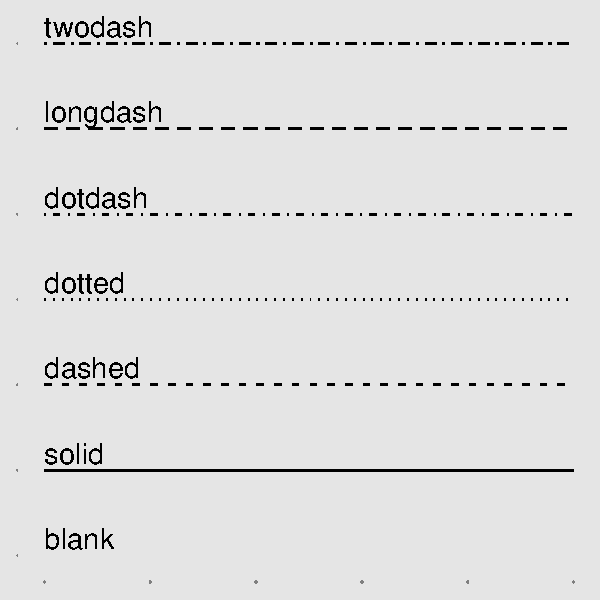
\includegraphics[width=0.5 \textwidth]{spec-linetype}
  \caption{Built-in line types.}
  \label{fig:linetype}
\end{figure}

Note that \code{NA} is not a valid value for \code{lty}.

\section{Shape}
\label{sec:shape_spec}

Shapes take four types of values:

\begin{itemize}
  \item Integer in $[0, 25]$.  These are illustrated in Figure~\ref{fig:shape}.

  \item A single character.  Can be a unicode charater, which 

  \item \code{.} is handled specially. In most devices, it draws the smallest shape that is visible (i.e. about one pixel).
  
  \item \code{NA}.  Point omitted.  
\end{itemize}

\begin{figure}[htbp]
  \centering
    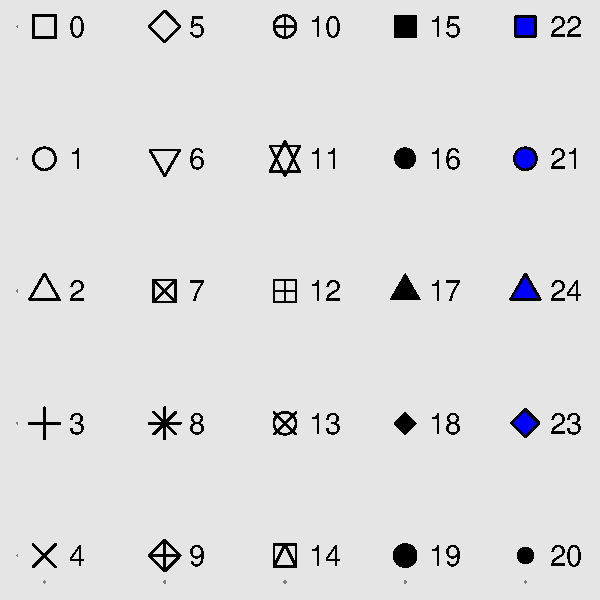
\includegraphics[width=0.5 \textwidth]{spec-shape}
  \caption{R plotting symbols.  Colour is black, and fill is blue.  Symbol 25 has been omitted from this plot, it is symbol 24 rotated 180 degrees.}
  \label{fig:shape}
\end{figure}

While all symbols have a foreground colour, symbols 19--25 also take a background colour (fill).  


\section{Justification}
\label{sec:justification_spec}

The justification of the text relative to its (x, y) location. If there are two values, the first value specifies horizontal justification and the second value specifies vertical justification. Possible string values are: \code{"left"}, \code{"right"}, \code{"centre"}, \code{"center"}, \code{"bottom"}, and \code{"top"}. For numeric values, 0 means left alignment and 1 means right alignment.

\begin{figure}[htbp]
  \centering
    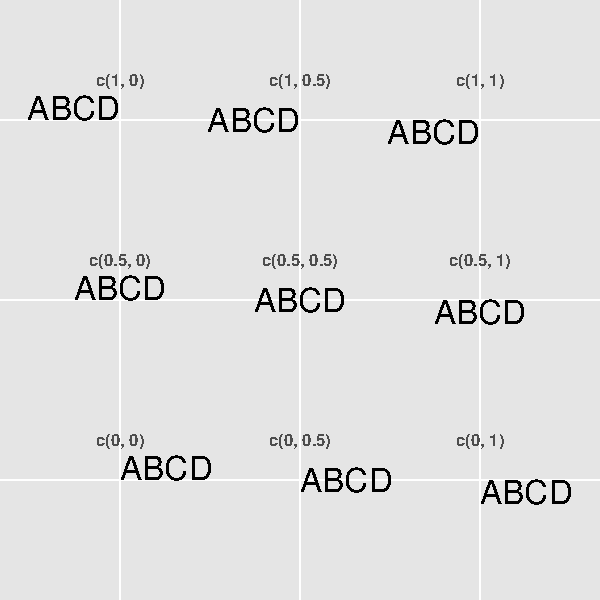
\includegraphics[width=0.5 \textwidth]{spec-justification}
  \caption{Horizontal and vertical justification settings.}
  \label{fig:justification}
\end{figure}

\ifwhole
\else
  \nobibliography{/Users/hadley/documents/phd/references}
  \end{document}
\fi